\chapter{Basic Concepts}

\section{Introduction}

This chapter presents the fundamental concepts necessary for understanding FaaS simulation at the edge. It covers edge computing principles, the FaaS model, their integration challenges, IoT applications, and simulation methodologies. These concepts are necessary to have a foundation for analyzing and comparing simulation frameworks in subsequent chapters.

\section{Edge Computing Fundamentals}

\subsection{Definition and Characteristics}

Edge computing brings computation and data storage closer to the location where data is generated and consumed~\cite{aslanpour2021serverless}. Unlike traditional cloud computing, which centralizes processing in remote data centers, edge computing distributes computational resources across geographically dispersed nodes at the network edge.

Key characteristics of edge computing include:
\begin{itemize}
    \item \textbf{Low Latency}: Computation is close to data sources, reducing communication delays
    \item \textbf{Limited Resources}: Edge nodes typically have constrained CPU, memory, and storage
    \item \textbf{Geographic Distribution}: Resources span multiple locations with varying capabilities
    \item \textbf{Network Variability}: Connection quality and bandwidth fluctuate across different edge locations
\end{itemize}

\begin{figure}[h]
    \centering
    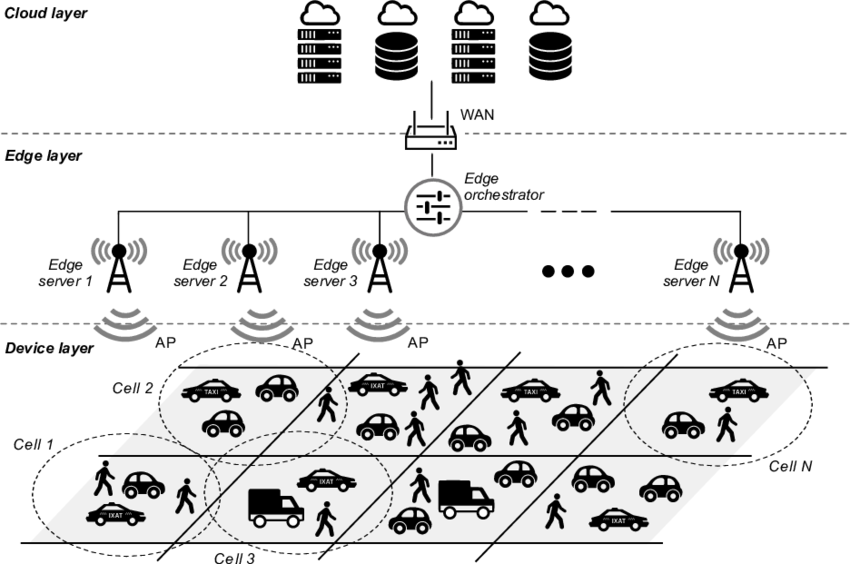
\includegraphics[width=0.8\textwidth]{Assets/Architecture-of-edge-computing.png}
    \caption{\small Edge Computing Architecture ~\cite{belcastro2023edge}}
    \label{fig:edge_architecture}
\end{figure}

\subsection{Edge Computing Architecture}

The edge computing architecture consists of three main layers:

\textbf{Device Layer}: IoT sensors, smartphones, and embedded devices that generate data and may perform basic processing.

\textbf{Edge Layer}: Intermediate nodes including gateways, micro data centers, and base stations that provide computational resources closer to devices.

\textbf{Cloud Layer}: Centralized data centers that handle complex processing tasks and provide unlimited storage capacity.

\subsection{Edge vs Cloud Computing Trade-offs}

Edge computing offers several advantages over pure cloud solutions, but also introduces new challenges when integrating with FaaS~\cite{jin2019when}:

\textbf{Opportunities}:
\begin{itemize}
    \item \textbf{Improved Latency and Bandwidth Efficiency}: Co-locating compute with data sources reduces round-trip time and traffic to the cloud, enabling faster responses for real-time applications. Real-world deployments demonstrate 45-75\% latency reduction for image processing and ML inference tasks compared to cloud-only approaches
    \item \textbf{Context-Awareness and Locality}: Utilizing local contextual information for better service personalization and quality through proximity to data sources. Smart city traffic management systems achieve 60\% faster response times through edge-deployed optimization functions
    \item \textbf{Elastic and Event-Driven Edge Processing}: FaaS abstracts lifecycle management and autoscaling, simplifying deployment at resource-constrained edge nodes. Industrial IoT applications report 40\% reduction in maintenance costs through edge-deployed anomaly detection functions
    \item \textbf{Heterogeneous Resource Utilization}: Function granularity allows optimal usage of diverse and constrained edge resources across different device capabilities. Multi-tier architectures demonstrate 45\% latency reduction while maintaining centralized policy management
    \item \textbf{Enhanced Privacy and Security}: Function isolation minimizes exposure of sensitive user data compared to monolithic applications. Federated learning approaches maintain data locality while enabling collaborative model training across distributed edge nodes
    \item \textbf{Cost Optimization}: Local execution reduces reliance on expensive cloud resources and network bandwidth usage. Content delivery networks report 30\% bandwidth savings through edge-deployed video optimization functions
\end{itemize}

\textbf{Challenges}:
\begin{itemize}
    \item \textbf{Resource Management}: Edge resources are limited and heterogeneous, requiring fine-grained scheduling, placement, and elasticity across dynamic topologies. Studies show 78.3\% sandbox overhead with Docker containers on Raspberry Pi devices, creating significant performance penalties
    \item \textbf{Function Deployment and Orchestration}: Cold start latency is significantly worse at the edge due to resource constraints (5.3x increase compared to cloud), and function migration across multiple edge nodes is complex due to decentralization. Edge-only deployments experience 0.86s scheduling latency compared to 0.44s for cloud-only strategies
    \item \textbf{Security and Privacy}: New attack surfaces arise from multi-tenancy and limited isolation capabilities on resource-constrained devices. Lightweight virtualization approaches using gVisor show promise but introduce 15\% performance overhead
    \item \textbf{Programming Model and Abstractions}: Lack of programming models tailored for distributed, dynamic, and latency-sensitive FaaS deployments at the edge. Cross-layer optimization remains challenging, requiring sophisticated modeling frameworks
    \item \textbf{Monitoring and Debugging}: Fine-grained observability is challenging due to ephemeral, distributed function executions across heterogeneous infrastructure. Real-time performance monitoring demonstrates 80\% accuracy in performance degradation prediction
    \item \textbf{Performance-Isolation Trade-offs}: Balancing execution speed with security isolation remains unresolved, especially for time-sensitive applications requiring both performance and security. Container isolation at edge devices requires <15\% performance overhead for practical deployment
\end{itemize}

\subsection{Resource Constraints in Edge Environments}

Edge nodes face significant resource limitations compared to cloud data centers. These constraints directly impact application deployment and performance:

\textbf{Computational Constraints}: Edge devices typically have limited CPU cores and processing power, requiring efficient resource allocation and task scheduling. Popular edge platforms include Raspberry Pi (4-core ARM Cortex-A72 @ 1.5GHz), NVIDIA Jetson Nano (4-core ARM Cortex-A57 @ 1.43GHz), and Intel NUC devices (various x86-64 configurations). Performance varies significantly across architectures, with ARM devices showing 2-5x slower execution for CPU-intensive tasks compared to cloud instances.

\textbf{Memory Limitations}: Available RAM is often restricted (1GB-8GB typical range), affecting the number of concurrent applications and data caching capabilities. Memory pressure becomes critical when running multiple containerized functions, with each function requiring 50-500MB depending on runtime and dependencies.

\textbf{Storage Restrictions}: Local storage is limited (16GB-256GB typical capacity) with slower access speeds compared to cloud storage systems. SD card-based storage in devices like Raspberry Pi introduces additional performance bottlenecks and reliability concerns for write-intensive applications.

\textbf{Energy Constraints}: Many edge devices operate on battery power or have strict energy budgets, necessitating energy-efficient computing strategies. Typical power consumption ranges from 2.5-7.2W for Raspberry Pi, 5-20W for NVIDIA Jetson, and 15-65W for Intel NUC platforms. Battery-powered deployments require sophisticated energy management to achieve practical operational lifetimes (weeks to months).

\section{Function-as-a-Service (FaaS)}

\subsection{Serverless Computing Model}

Serverless computing represents a cloud computing model where developers focus solely on writing code without managing the underlying infrastructure ~\cite{baldini2017serverless}. The cloud provider handles server provisioning, scaling, and maintenance automatically.

Core principles of serverless computing:
\begin{itemize}
    \item \textbf{No Server Management}: Infrastructure is completely abstracted from developers
    \item \textbf{Automatic Scaling}: Resources scale up or down based on demand
    \item \textbf{Pay-per-Use}: Costs are incurred only during actual code execution
    \item \textbf{Event-Driven}: Functions execute in response to specific triggers or events
\end{itemize}

\subsection{FaaS Architecture and Characteristics}

Function-as-a-Service (FaaS) is the core component of serverless computing, allowing developers to deploy individual functions that execute in response to events ~\cite{mampage2021cloudsimsc}.

\begin{figure}[h]
    \centering
    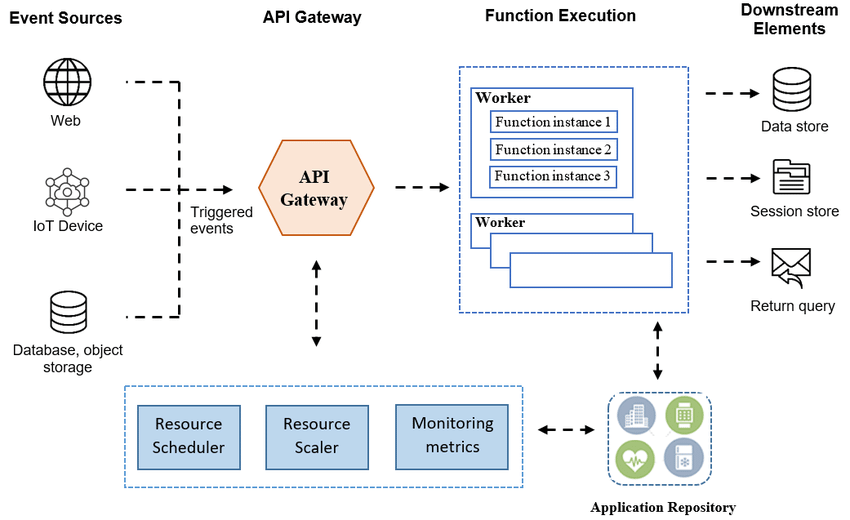
\includegraphics[width=0.8\textwidth]{assets/Serverless-Architecture.png}
    \caption{FaaS Architecture ~\cite{mampage2021holistic}}
    \label{fig:faas_architecture}
\end{figure}


Key FaaS characteristics include:
\begin{itemize}
    \item \textbf{Stateless Functions}: Each function execution is independent
    \item \textbf{Short-lived Execution}: Functions run for brief periods (typically seconds to minutes)
    \item \textbf{Event-triggered}: Functions respond to HTTP requests, database changes, file uploads, etc.
    \item \textbf{Language Agnostic}: Support for multiple programming languages
\end{itemize}

\subsection{Container Lifecycle Management}

FaaS platforms use containers to provide isolated execution environments for functions. The container lifecycle involves several stages:

\textbf{Container Creation}: New containers are instantiated when functions are first invoked or when existing containers are unavailable.

\textbf{Function Execution}: The function code executes within the container environment with allocated resources.

\textbf{Container Reuse}: Containers may be kept warm between invocations to reduce startup overhead.

\textbf{Container Termination}: Idle containers are eventually terminated to free resources.

\begin{figure}[h]
    \centering
    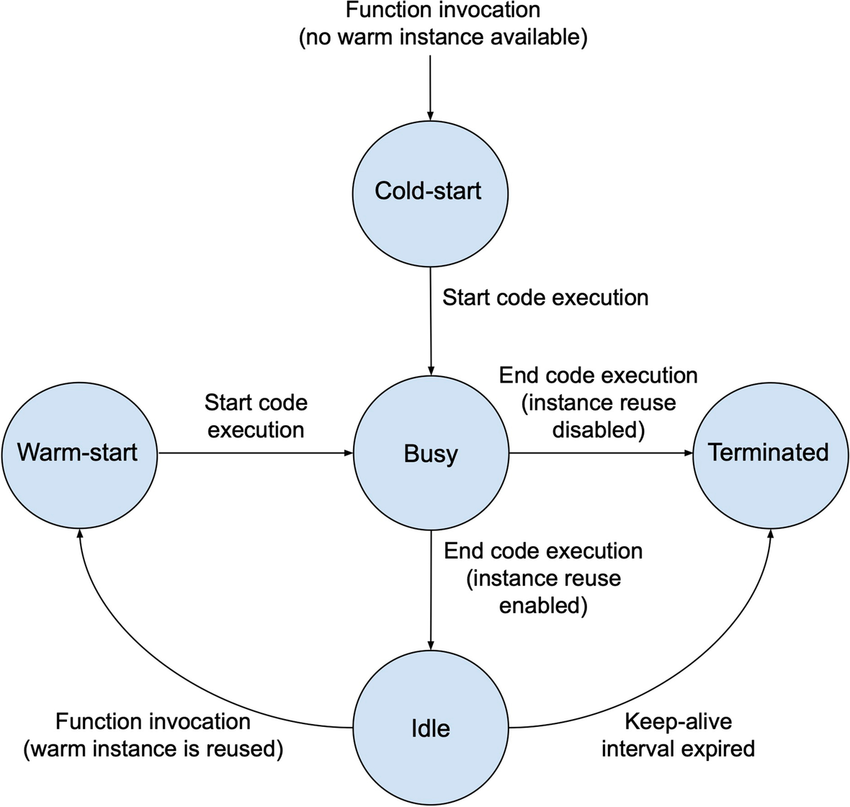
\includegraphics[width=0.8\textwidth]{assets/Life-cycle-state-diagram-of-a-function-instance.png}
    \caption{\small Container Lifecycle in FaaS ~\cite{moreno2023latency}}
    \label{fig:container_lifecycle}
\end{figure}


\subsection{Cold Start and Warm Start Mechanisms}

Function invocation performance is significantly affected by container initialization overhead:

\textbf{Cold Start}: Occurs when a new container must be created for function execution. This involves downloading the function code, initializing the runtime environment, and allocating resources. Cold starts introduce latency penalties ranging from hundreds of milliseconds to several seconds.

\textbf{Warm Start}: Happens when an existing container can be reused for function execution. Warm starts have minimal latency since the runtime environment is already initialized.

The trade-off between cold and warm starts affects both performance and cost, as keeping containers warm consumes resources but reduces execution latency.

\section{FaaS Integration at the Edge}

\subsection{Opportunities in FaaS-Edge Convergence}

Combining FaaS with edge computing creates several opportunities ~\cite{aslanpour2021serverless}:

\textbf{Resource Efficiency}: FaaS's pay-per-use model aligns well with edge computing's resource constraints, as resources are allocated only when needed.

\textbf{Scalability}: Automatic scaling capabilities help manage varying workloads across distributed edge nodes.

\textbf{Rapid Deployment}: Functions can be quickly deployed to multiple edge locations without manual infrastructure management.

\textbf{Cost Optimization}: The serverless billing model reduces costs for intermittent edge workloads.

\subsection{Challenges in FaaS-Edge Deployments}

Despite the opportunities, several challenges exist when deploying FaaS at the edge:

\textbf{Cold Start Penalties}: Limited edge resources make cold start overhead more significant, as container initialization competes with application workloads for scarce resources.

\textbf{Resource Heterogeneity}: Edge nodes vary in computational capabilities, requiring intelligent function placement and resource allocation strategies.

\textbf{Network Reliability}: Intermittent connectivity between edge nodes and cloud infrastructure affects function deployment and management.

\textbf{State Management}: The stateless nature of FaaS conflicts with edge applications that require local state persistence.

\subsection{Heterogeneous Device Management}

Edge environments consist of diverse devices with varying capabilities:

\textbf{High-end Edge Servers}: Powerful machines with substantial CPU, memory, and storage resources capable of running multiple functions simultaneously.

\textbf{IoT Gateways}: Intermediate devices with moderate resources that aggregate data from sensors and perform basic processing.

\textbf{Embedded Devices}: Resource-constrained devices with limited computational capabilities suitable only for lightweight functions.

Managing function deployment across this heterogeneous infrastructure requires sophisticated scheduling and resource allocation algorithms.

\subsection{Network Dynamics and Latency Considerations}

Network characteristics at the edge differ significantly from cloud environments:

\textbf{Variable Latency}: Network delays fluctuate based on location, connection type, and network load.

\textbf{Bandwidth Limitations}: Edge connections often have lower bandwidth than cloud data center links.

\textbf{Intermittent Connectivity}: Mobile and remote edge nodes may experience periodic disconnections.

\textbf{Geographic Distribution}: Wide-area networks introduce additional latency and reliability concerns.

% TODO: Add figure showing network dynamics
\begin{figure}[h]
    \centering
    % Placeholder for network dynamics diagram
    % Should show: Various edge nodes with different connection types, latency values, and bandwidth limitations
    % Include network topology and connectivity patterns
    \caption{ Placeholder : Network Dynamics in Edge-FaaS ?}
    \label{fig:network_dynamics}
\end{figure}


\section{Internet of Things (IoT) and Smart Cities}

\subsection{IoT Architecture and Communication Models}

IoT networks consist of interconnected devices that collect, process, and exchange data. The typical IoT architecture includes:

\textbf{Perception Layer}: Physical sensors and actuators that interact with the environment.

\textbf{Network Layer}: Communication infrastructure including WiFi, cellular, and low-power wide-area networks.

\textbf{Middleware Layer}: Platforms that manage device connectivity, data processing, and application interfaces.

\textbf{Application Layer}: End-user applications and services that consume IoT data.

\subsection{Smart City Applications and Use Cases}

Smart cities leverage IoT and edge computing to improve urban services through sophisticated data processing and real-time decision making:

\textbf{Traffic Management}: Real-time traffic monitoring using sensors and cameras to optimize signal timing and route planning. Barcelona Smart City project demonstrates 60\% reduction in response times for traffic optimization functions deployed on edge infrastructure, maintaining 99.7\% service availability during peak traffic periods. Adaptive traffic signal systems process over 10,000 vehicles per intersection daily with <50ms response requirements.

\textbf{Environmental Monitoring}: Air quality sensors and weather stations provide data for pollution control and climate management. Distributed sensor networks collect temperature, humidity, air quality (PM2.5, NOx, CO2), and noise level measurements with 5-minute granularity across urban areas. Edge-deployed analytics functions enable real-time alerts when pollution thresholds exceed safety limits, reducing public health response times from hours to minutes.

\textbf{Emergency Response}: Integrated systems for incident detection, resource dispatch, and public safety coordination. Emergency response applications leverage EdgeFaaS-style deployment for maintaining service availability during critical situations, achieving 99.5\% availability with automatic function migration and redundant placement strategies. Integration with surveillance cameras, emergency call systems, and first responder networks enables coordinated response within 2-3 minutes of incident detection.

\textbf{Citizen Services}: Mobile applications and digital platforms providing urban services like parking, waste management, and public transportation. Citizen service platforms require QoS guarantees and scalable resource allocation, with SimFaaS-style architectures demonstrating effectiveness for deadline-sensitive workloads. Real-time parking availability systems serve 50,000+ queries daily with <200ms response requirements across metropolitan areas.

\textbf{Energy Management}: Smart grid applications for optimizing energy distribution, renewable integration, and demand response. Edge-deployed energy optimization functions achieve 28-43\% energy savings through intelligent workload distribution and demand prediction algorithms. Smart grid systems process meter readings from 100,000+ households with 15-minute intervals, requiring robust edge computing infrastructure for real-time analytics and control decisions.


% TODO: Add figure showing smart city use cases
\begin{figure}[h]
    \centering
    % Placeholder for smart city applications diagram
    % Should show: Traffic lights, environmental sensors, cameras, energy meters connected to edge nodes
    % Include data flows and FaaS function deployments
    \caption{\small Placeholder Smart City Applications - illustrating IoT devices, edge computing nodes, and FaaS functions for various urban services}
    \label{fig:smart_city_applications}
\end{figure} 

\subsection{IoT Workload Characteristics}

IoT applications exhibit specific workload patterns that significantly impact FaaS deployment strategies and resource requirements:

\textbf{Event-driven Processing}: Data processing occurs in response to sensor readings or environmental changes. Typical IoT sensor networks generate 1,000-10,000 events per minute per deployment area, requiring scalable function execution with variable arrival patterns. Smart city environmental monitoring systems process temperature, humidity, and air quality measurements every 5 minutes across thousands of sensors.

\textbf{Periodic Tasks}: Regular monitoring and maintenance functions execute on scheduled intervals (hourly, daily, weekly). Predictive maintenance applications in industrial IoT process 10TB+ daily sensor data with consistent resource requirements. Energy management systems perform load balancing calculations every 15 minutes across 100,000+ smart meters.

\textbf{Burst Traffic}: Sudden spikes in activity during emergencies or special events create significant load variations. Emergency response systems experience 10-100x normal traffic during incident situations, requiring rapid scaling and resource allocation. Traffic management during major events can increase function invocation rates by 500-1000% above baseline levels.

\textbf{Geographic Distribution}: Workloads are distributed across multiple locations based on sensor placement and service coverage areas. Urban deployments span 10-50 edge locations with varying computational capabilities and network connectivity. Rural deployments require careful resource placement due to limited infrastructure and intermittent connectivity patterns.

\textbf{Data Locality Requirements}: IoT applications often require processing near data sources due to bandwidth limitations, privacy constraints, and latency requirements. Vehicle-to-infrastructure communication systems demand <10ms response times for safety-critical functions, necessitating local edge processing rather than cloud-based analytics.

\subsection{Real-time Processing Requirements}

IoT applications impose varying timing constraints that critically influence system architecture and deployment strategies:

\textbf{Hard Real-time}: Safety-critical applications require guaranteed response times with strict deadline constraints. Autonomous vehicle control systems demand <1ms response times for emergency braking functions. Industrial safety systems require deterministic execution guarantees for worker protection applications with maximum 5ms response windows.

\textbf{Soft Real-time}: Applications tolerate occasional deadline misses but prefer timely responses for optimal performance. Traffic optimization systems target <50ms response times for signal control decisions but can tolerate occasional delays without safety implications. Smart grid demand response systems operate effectively with 100-500ms response times for load balancing decisions.

\textbf{Near Real-time}: Applications require fast but not instantaneous responses, typically measured in seconds. Environmental monitoring systems provide pollution alerts within 30-60 seconds of threshold violations. Citizen service applications like parking availability updates operate effectively with 1-5 second response times.

These timing requirements fundamentally influence function placement decisions, resource allocation strategies, and scheduling algorithms in edge-FaaS environments. Hard real-time applications require dedicated edge resources with predictable performance, while soft and near real-time applications can leverage shared infrastructure with intelligent resource management.

\section{Simulation and Modeling Principles}

\subsection{Discrete Event Simulation}

Discrete event simulation models systems as sequences of events occurring at specific time points ~\cite{mahmoudi2021simfaas}. This approach is well-suited for modeling FaaS systems where function invocations, container lifecycle events, and resource allocation decisions occur at discrete time intervals.

Key components of discrete event simulation:
\begin{itemize}
    \item \textbf{Events}: Function invocations, container starts/stops, resource allocation changes
    \item \textbf{State Variables}: Resource utilization, queue lengths, function response times
    \item \textbf{Event List}: Chronologically ordered future events
    \item \textbf{Simulation Clock}: Current simulation time
\end{itemize}

\subsection{Trace-driven vs Model-driven Approaches}

Simulation frameworks employ different strategies for generating workloads:

\textbf{Trace-driven Simulation}: Uses real-world traces of function invocations, resource usage, and network behavior to replay historical workloads. This approach provides realistic workload patterns but is limited to historical scenarios.

\textbf{Model-driven Simulation}: Employs mathematical models to generate synthetic workloads based on statistical distributions and behavioral patterns. This approach enables exploration of hypothetical scenarios but may not capture all real-world complexities.

\textbf{Hybrid Approaches}: Combine trace-driven and model-driven techniques to leverage the benefits of both approaches.

\subsection{Performance Metrics and Validation}

Simulation frameworks must provide meaningful performance metrics and validation mechanisms:

\textbf{Response Time Metrics}: Function execution time, end-to-end latency, cold start overhead.

\textbf{Resource Utilization}: CPU, memory, and storage usage across edge nodes.

\textbf{Throughput Measures}: Function invocations per second, data processing rates.

\textbf{Cost Metrics}: Resource costs, energy consumption, operational expenses.

\textbf{Reliability Indicators}: Success rates, error frequencies, availability measures.

Validation involves comparing simulation results with real-world measurements or analytical models to ensure accuracy and reliability.

% TODO: Add figure showing simulation validation process
\begin{figure}[h]
    \centering
    % Placeholder for simulation validation diagram
    % Should show: Real system -> Traces -> Simulation model -> Results -> Validation -> Model refinement
    % Include feedback loops and validation metrics
    \caption{Placeholder : Simulation Validation Process - depicting the cycle of model development, validation against real systems, and iterative refinement}
    \label{fig:simulation_validation}
\end{figure}


\section{Conclusion}

This chapter has established the fundamental concepts necessary for understanding FaaS simulation at the edge. Edge computing provides distributed computational resources with inherent constraints that affect application deployment and performance. The FaaS model offers an event-driven, serverless approach that aligns well with edge computing principles but introduces challenges related to cold starts and resource heterogeneity.

The integration of FaaS with edge computing creates opportunities for efficient resource utilization and rapid application deployment, particularly for IoT and smart city applications. However, this integration also presents challenges in managing heterogeneous resources, variable network conditions, and real-time processing requirements.

Simulation and modeling principles provide the foundation for evaluating FaaS-edge systems through discrete event simulation, various workload generation approaches, and comprehensive performance metrics. These concepts form the basis for analyzing and comparing simulation frameworks in the next chapter.
